\documentclass[11pt]{article}

% -------------------- Packages --------------------
\usepackage[margin=1in]{geometry}
\usepackage{array}
\usepackage{longtable}
\usepackage{graphicx}
\usepackage{enumitem}
\usepackage{caption}
\usepackage{titlesec}
\usepackage{float}
\usepackage{booktabs}
\usepackage{xcolor}

% -------------------- Formatting --------------------
\setlist[itemize]{noitemsep, topsep=0pt}
\setlength{\parskip}{0.5em}
\setlength{\parindent}{0pt}

\captionsetup{
    justification=centering,
    labelfont=bf,
    textfont=normalfont
}

% Section formatting
\titleformat{\section}
{\normalfont\Large\bfseries}{\thesection}{1em}{}

% -------------------- Document --------------------
\begin{document}

% -------------------- Header --------------------
\begin{center}
    {\Large\bfseries Sri Sivasubramaniya Nadar College of Engineering, Chennai}\\[0.3em]
    {\bfseries (An Autonomous Institution affiliated to Anna University)}
\end{center}


% -------------------- Details Table --------------------
\begin{table}[h]
\renewcommand{\arraystretch}{1.4}
\resizebox{\textwidth}{!}{%
\begin{tabular}{|l|l|l|l|}
\hline
Degree \& Branch & B.E. Computer Science \& Engineering & Semester & VI \\ \hline
Subject Code \& Name & \multicolumn{3}{l|}{UCS2612 – Machine Learning Algorithms Laboratory} \\ \hline
Academic Year & 2025–2026 (Even) & Batch & 2023–2027 \\ \hline
Name & Kushaal Shyam Potta & Register No. & 3122235001071 \\ \hline
Due Date & \multicolumn{3}{l|}{09.01.2026} \\ \hline
\end{tabular}}
\end{table}

% -------------------- Title --------------------
\begin{center}
    {\Large\bfseries Experiment 2: Binary Classification using Naïve Bayes and K-Nearest Neighbors}
\end{center}



% --------------------------------------------------
\section{Aim and Objective}
To build and evaluate Naïve Bayes (Gaussian, Multinomial, and Bernoulli) and K-Nearest Neighbors (KNN) classifiers for the binary classification task of spam detection. The experiment involves data preprocessing, exploratory data analysis, hyperparameter tuning using Grid and Randomized search, and performance comparison using metrics such as Accuracy, Precision, Recall, F1-Score, and Specificity.

% --------------------------------------------------
\section{Dataset Description}
The experiment utilizes the \textbf{Spambase} dataset, which consists of features extracted from emails to classify them as spam or non-spam.

\begin{itemize}
    \item \textbf{Total Instances:} 4601 (Original), 4210 (After removing duplicates)
    \item \textbf{Total Features:} 57 numerical features (word frequencies, character frequencies, run length attributes) + 1 target class
    \item \textbf{Target Variable:} `class' (1 for Spam, 0 for Non-Spam)
\end{itemize}

\textbf{Dataset Reference:} Kaggle -- Spambase Dataset

% --------------------------------------------------
\section{Preprocessing Steps}
\begin{itemize}
    \item \textbf{Data Loading:} The dataset was loaded using the Pandas library.
    \item \textbf{Duplicate Removal:} 391 duplicate rows were identified and removed to ensure data quality, reducing the dataset size to 4210 instances.
    \item \textbf{Feature Scaling:} The \texttt{StandardScaler} was applied to normalize the features for Gaussian Naïve Bayes and KNN models. Multinomial Naïve Bayes utilized the original non-negative features.
    \item \textbf{Train-Test Split:} The data was split into training and testing sets to evaluate model performance on unseen data.
\end{itemize}

% --------------------------------------------------
\section{Implementation Details}

\subsection{Naïve Bayes}
Three variants were implemented:
\begin{itemize}
    \item \textit{GaussianNB:} Applied to scaled data for continuous features.
    \item \textit{MultinomialNB:} Applied to raw count/frequency data.
    \item \textit{BernoulliNB:} Applied to binary/boolean feature representations.
\end{itemize}

\subsection{K-Nearest Neighbors (KNN)}
\begin{itemize}
    \item A baseline KNN model was trained.
    \item \textbf{Hyperparameter Tuning:} \texttt{GridSearchCV} and \texttt{RandomizedSearchCV} were used to find the optimal $k$ value, distance metric, and weight function.
    \item \textbf{Search Algorithms:} Evaluated using \textit{KDTree} and \textit{BallTree} structures for efficiency.
\end{itemize}

% --------------------------------------------------
\section{Visualizations}

\begin{figure}[H]
    \centering
    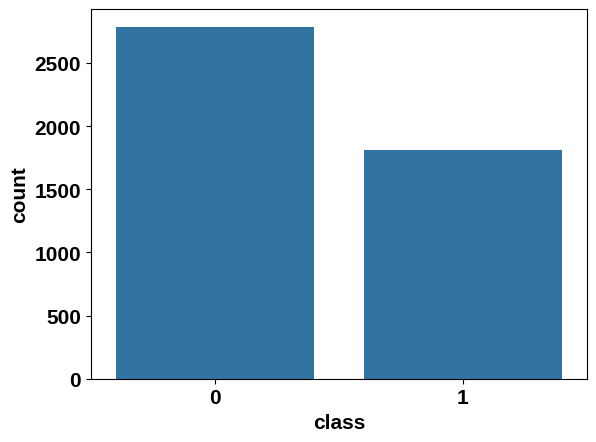
\includegraphics[width=0.65\textwidth]{spam_class_distribution.png}
    \caption{Class Distribution of Spam and Non-Spam Emails}
    \label{fig:class_dist}
\end{figure}

\begin{figure}[H]
    \centering
    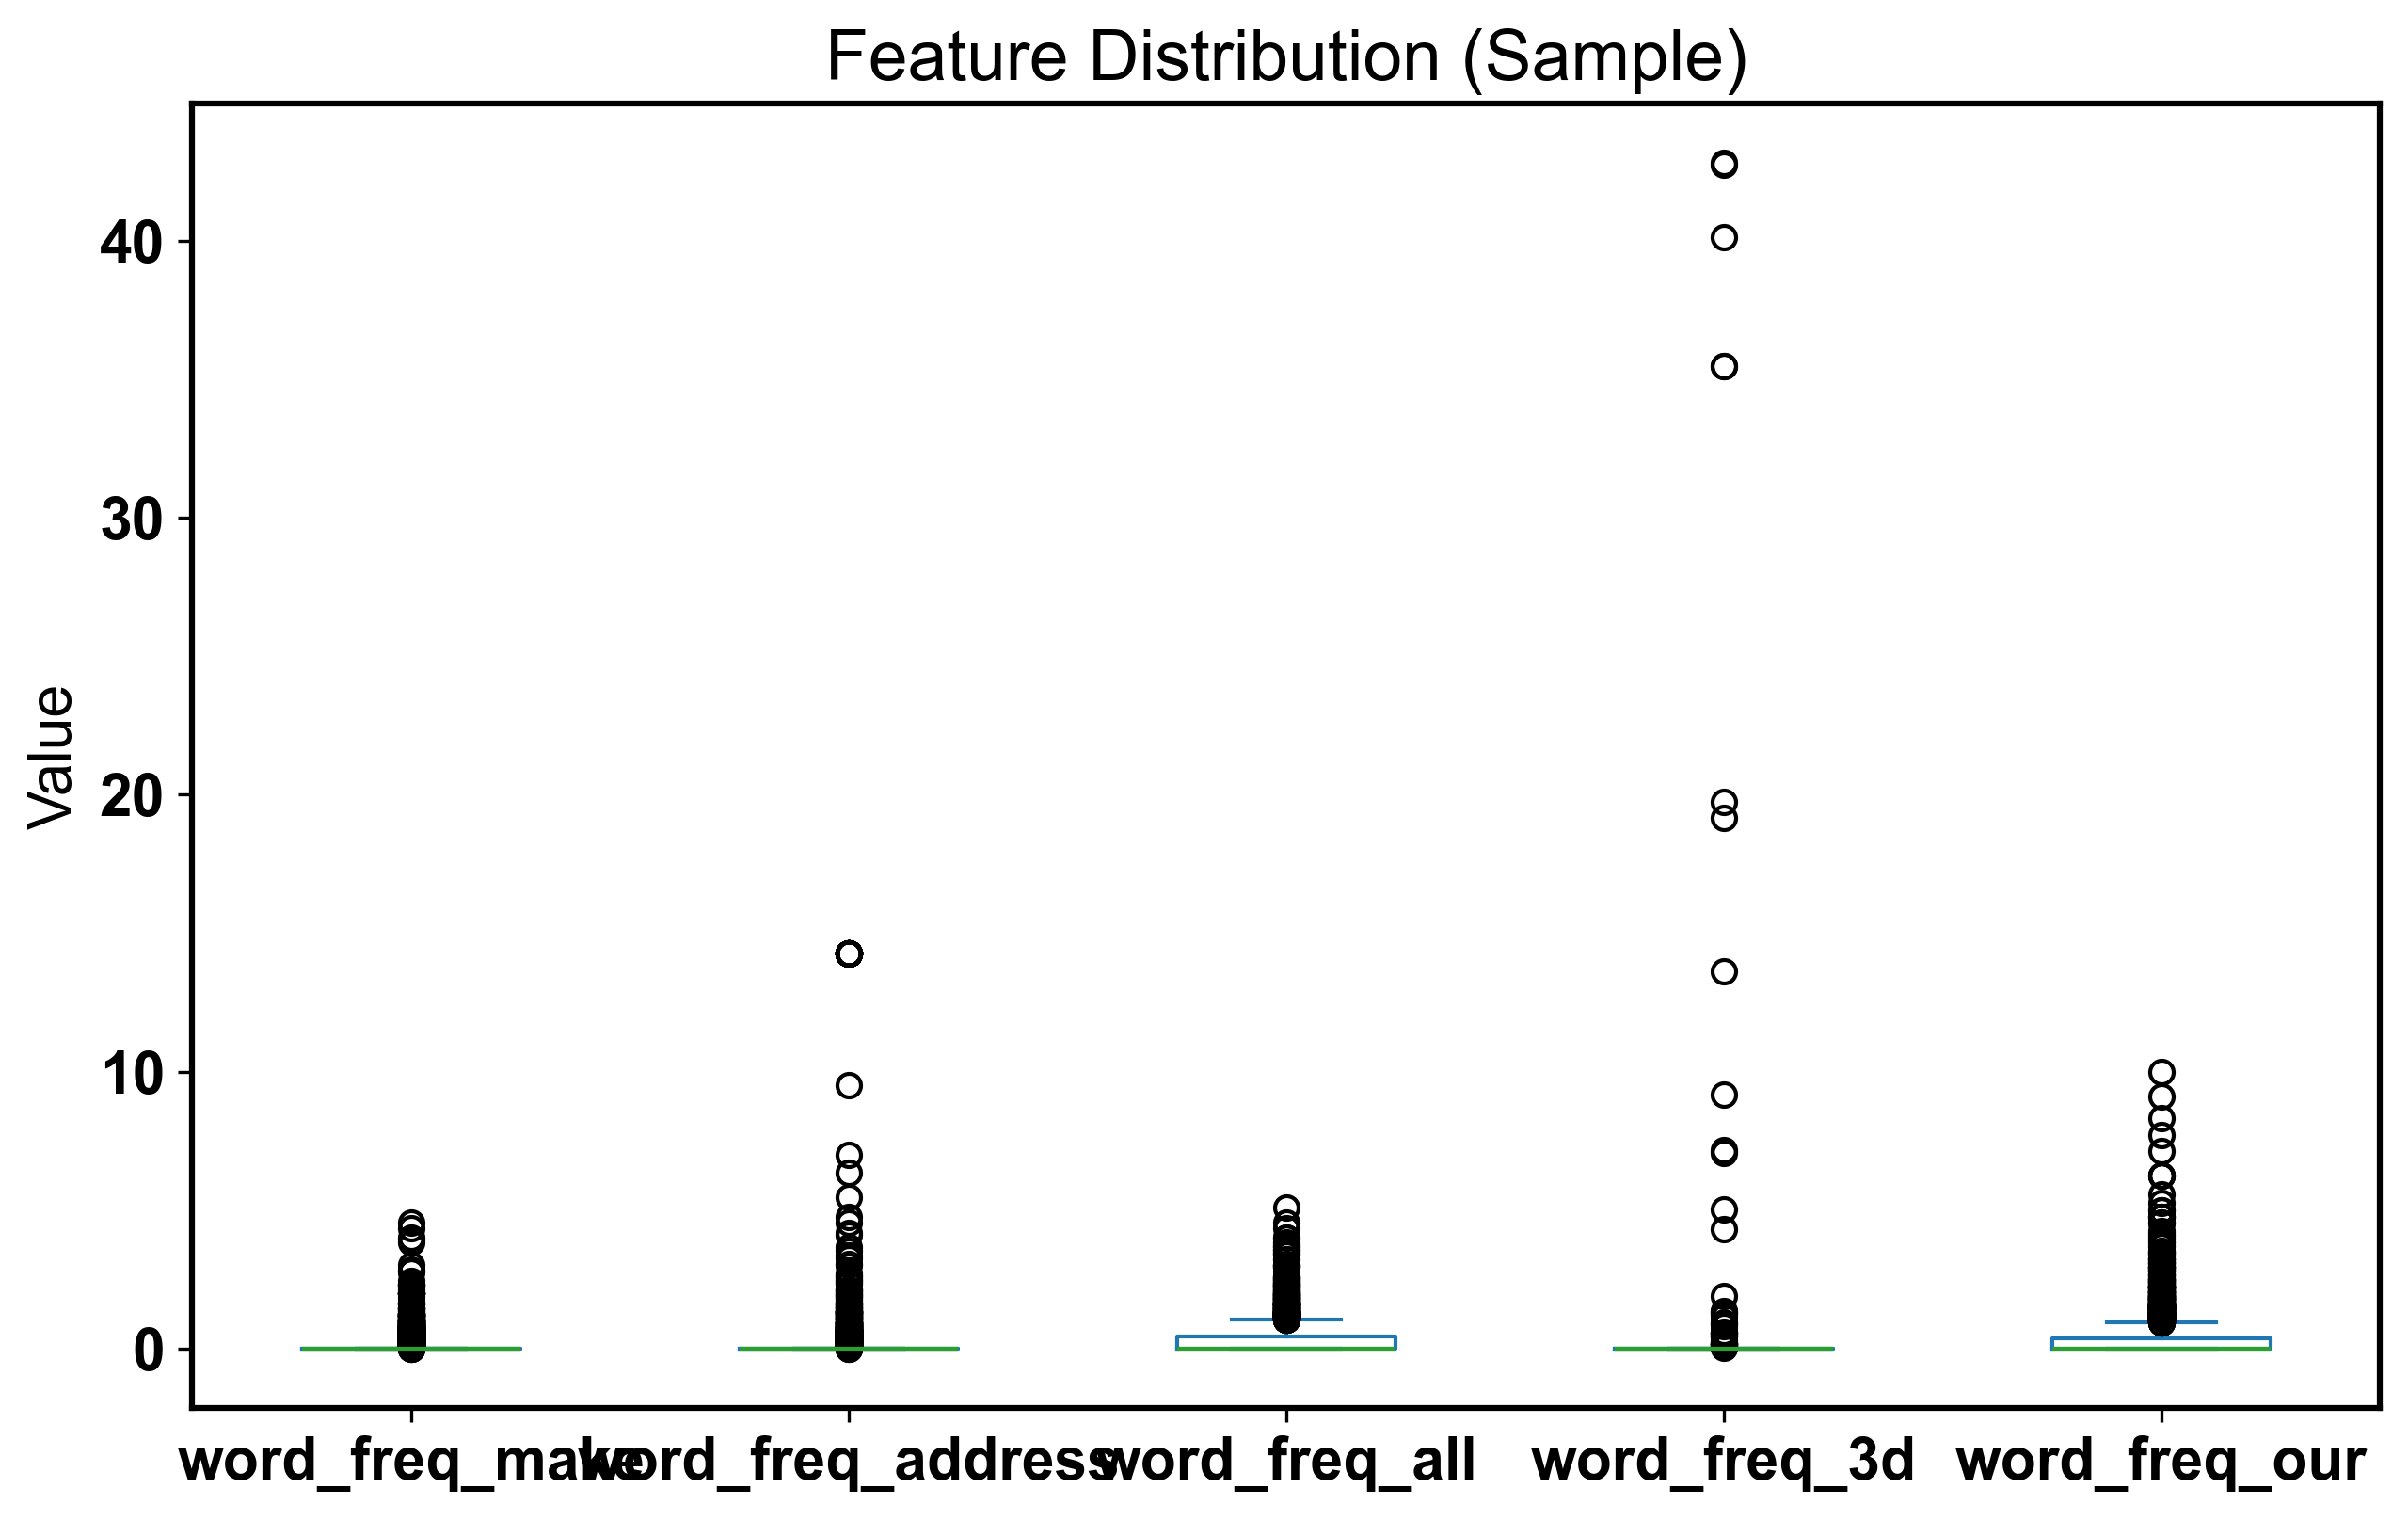
\includegraphics[width=0.85\textwidth]{feature_distribution.png}
    \caption{Feature Distribution Plot (Box plot)}
    \label{fig:feature_box}
\end{figure}

\begin{figure}[H]
    \centering
    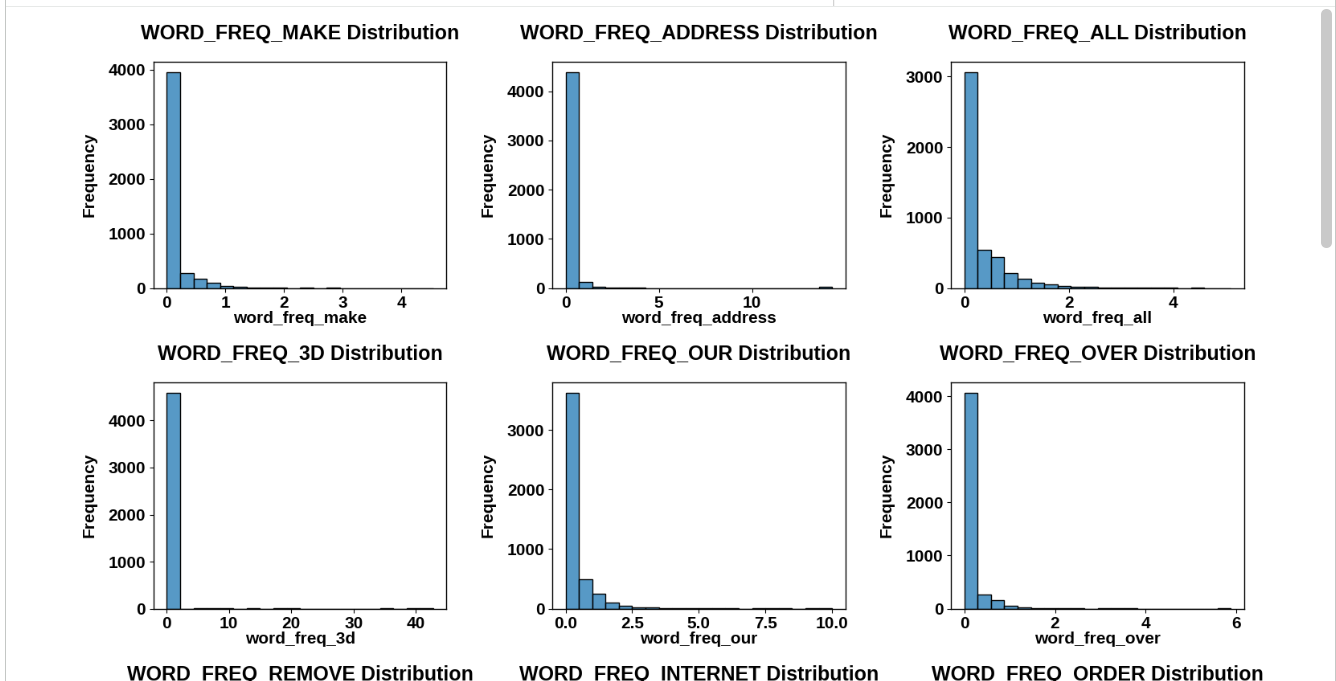
\includegraphics[width=0.85\textwidth]{spam_hist_distribution.png}
    \caption{Feature Distribution Plot (Histogram)}
    \label{fig:feature_hist}
\end{figure}

\begin{figure}[H]
    \centering
    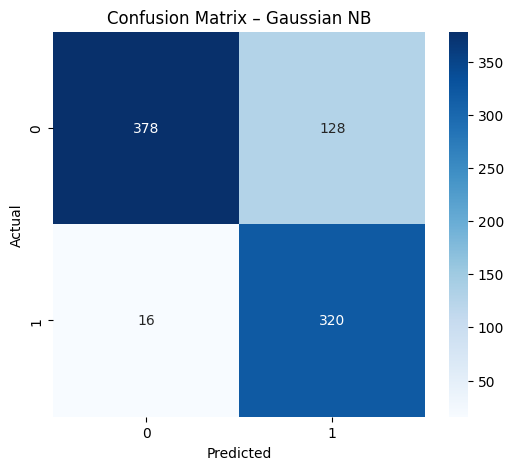
\includegraphics[width=0.55\textwidth]{confusion_matrix_gnb.png}
    \caption{Confusion Matrix for Gaussian Naïve Bayes}
    \label{fig:cm_gnb}
\end{figure}

\begin{figure}[H]
    \centering
    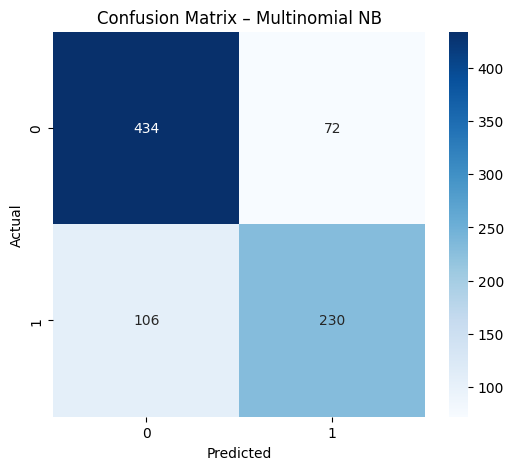
\includegraphics[width=0.55\textwidth]{confusion_matrix_mnb.png}
    \caption{Confusion Matrix for Multinomial Naïve Bayes}
    \label{fig:cm_mnb}
\end{figure}

\begin{figure}[H]
    \centering
    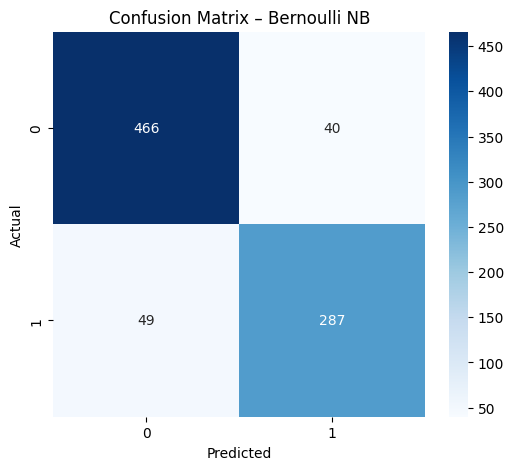
\includegraphics[width=0.55\textwidth]{confusion_matrix_bnb.png}
    \caption{Confusion Matrix for Bernoulli Naïve Bayes}
    \label{fig:cm_bnb}
\end{figure}

\begin{figure}[H]
    \centering
    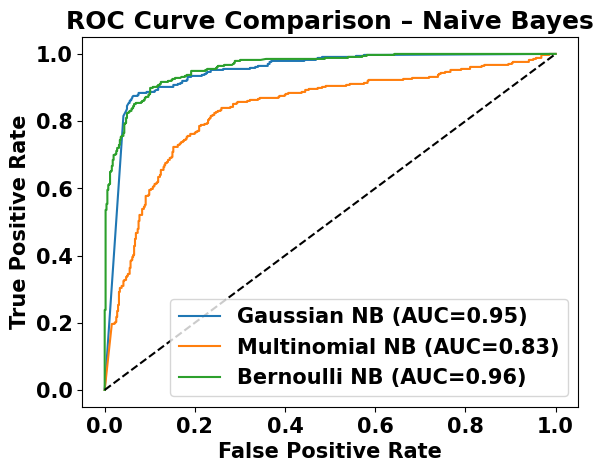
\includegraphics[width=0.65\textwidth]{roc_nb.png}
    \caption{ROC Curve for Naïve Bayes Models}
    \label{fig:roc_nb}
\end{figure}

\begin{figure}[H]
    \centering
    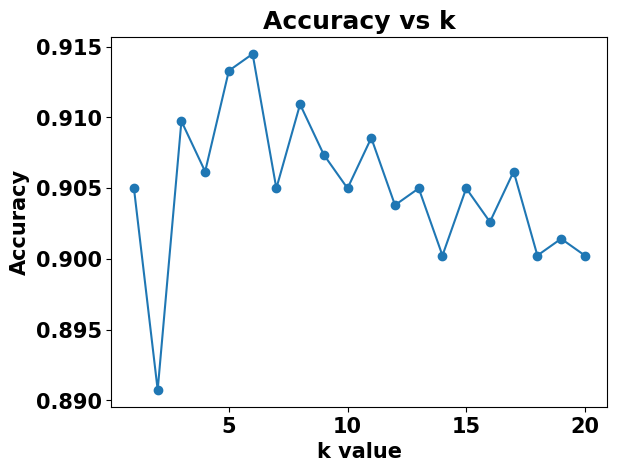
\includegraphics[width=0.7\textwidth]{accuracyvsk.png}
    \caption{Accuracy vs. $k$ Plot for KNN}
    \label{fig:acc_vs_k}
\end{figure}

\begin{figure}[H]
    \centering
    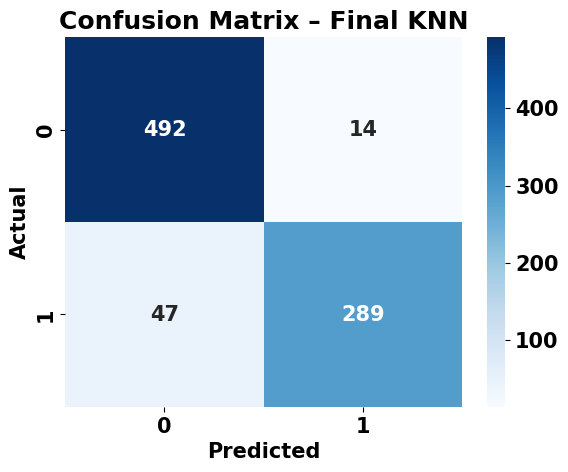
\includegraphics[width=0.7\textwidth]{confusion_matrix_knn.png}
    \caption{Confusion Matrix for Final KNN}
    \label{fig:cm_knn}
\end{figure}

% --------------------------------------------------
\section{Performance Tables}

\begin{table}[H]
\centering
\caption{Naïve Bayes Performance Metrics}
\begin{tabular}{|l|c|c|c|}
\hline
\textbf{Metric} & \textbf{Gaussian NB} & \textbf{Multinomial NB} & \textbf{Bernoulli NB} \\ \hline
Accuracy & 0.8290 & 0.7886 & 0.8943 \\ \hline
Precision & 0.7143 & 0.7616 & 0.8777 \\ \hline
Recall & 0.9524 & 0.6845 & 0.8542 \\ \hline
F1 Score & 0.8163 & 0.7210 & 0.8658 \\ \hline
Specificity & 0.7470 & 0.8577 & 0.9209 \\ \hline
Training Time (s) & 0.0031 & 0.0033 & 0.0043 \\ \hline
\end{tabular}
\end{table}

\begin{table}[H]
\centering
\caption{KNN Hyperparameter Tuning}
\begin{tabular}{|l|c|c|}
\hline
\textbf{Search Method} & \textbf{Best Parameters} & \textbf{Best CV Accuracy} \\ \hline
Grid Search & k=7, weights='distance', metric='manhattan' & 0.9181 \\ \hline
Randomized Search & k=6, weights='distance', metric='manhattan' & 0.9127 \\ \hline
\end{tabular}
\end{table}

\begin{table}[H]
\centering
\caption{KNN Performance using KDTree (Final Model)}
\begin{tabular}{|l|c|}
\hline
\textbf{Metric} & \textbf{Value} \\ \hline
Optimal k & 7 \\ \hline
Accuracy & 0.9276 \\ \hline
Precision & 0.9538 \\ \hline
Recall & 0.8601 \\ \hline
F1 Score & 0.9045 \\ \hline
Training Time (s) & 0.0013 \\ \hline
Prediction Time (s) & 0.0179 \\ \hline
\end{tabular}
\end{table}

\begin{table}[H]
\centering
\caption{KNN Performance using BallTree (Final Model)}
\begin{tabular}{|l|c|}
\hline
\textbf{Metric} & \textbf{Value} \\ \hline
Optimal k & 7 \\ \hline
Accuracy & 0.9276 \\ \hline
Precision & 0.9538 \\ \hline
Recall & 0.8601 \\ \hline
F1 Score & 0.9045 \\ \hline
Training Time (s) & 0.0013 \\ \hline
Prediction Time (s) & 0.0179 \\ \hline
\end{tabular}
\end{table}

\begin{table}[H]
\centering
\caption{Comparison of Neighbor Search Algorithms}
\begin{tabular}{|l|c|c|}
\hline
\textbf{Criterion} & \textbf{KDTree} & \textbf{BallTree} \\ \hline
Accuracy & 0.9276 & 0.9276 \\ \hline
Training Time (s) & 0.0013 & 0.0013 \\ \hline
Prediction Time (s) & 0.0179 & 0.0179 \\ \hline
Memory Usage & Low / Medium & Medium / High \\ \hline
\end{tabular}
\end{table}


% --------------------------------------------------
\section{Overfitting and Underfitting Analysis}
\begin{itemize}
    \item \textbf{Underfitting:} Observed in Multinomial Naïve Bayes, where the assumption of feature independence and integer counts may not fully capture the complexity of the continuous features in the dataset, leading to lower recall (0.6845).
    \item \textbf{Overfitting:} In KNN, very small values of $k$ (e.g., $k=1$) often lead to overfitting as the model becomes too sensitive to noise in the training data. The grid search identified $k=7$ as optimal, balancing bias and variance.
    \item \textbf{Optimal Balance:} The Bernoulli NB and Optimized KNN models showed robust performance on the test set (Accuracy $>$ 89\%), indicating good generalization without significant overfitting.
\end{itemize}

% --------------------------------------------------
\section{Bias--Variance Analysis}
\begin{itemize}
    \item \textbf{Gaussian NB:} High Recall (0.9524) but lower Precision (0.7143) indicates the model is biased towards the positive class (Spam), capturing most spam emails but with more false positives.
    \item \textbf{Multinomial NB:} Lower Recall (0.6845) suggests high bias against the spam class structure in this specific feature set.
    \item \textbf{KNN:} The distance-weighted KNN with Manhattan distance ($k=7$) achieved the highest Specificity (0.9723) and F1 Score (0.9045), demonstrating low bias and low variance after tuning.
\end{itemize}

% --------------------------------------------------
\section{Observations and Conclusion}
The experiment demonstrated that for the Spambase dataset:
\begin{itemize}
    \item \textbf{KNN (Tuned)} outperformed all Naïve Bayes variants with an accuracy of \textbf{92.76\%} and an F1-score of \textbf{0.9045}.
    \item Among Naïve Bayes classifiers, \textbf{Bernoulli NB} performed best (Accuracy: 89.43\%), suggesting that the presence/absence of words is a strong predictor for spam.
    \item Hyperparameter tuning significantly improved KNN performance, with \texttt{GridSearchCV} identifying Manhattan distance and distance-based weights as optimal.
    \item Gaussian NB showed the highest Recall, making it suitable if the cost of missing a spam email is high, though at the cost of precision.
\end{itemize}

% --------------------------------------------------
\section{References}
\begin{enumerate}
    \item Scikit-learn -- Naïve Bayes Documentation
    \item Scikit-learn -- KNN Documentation
    \item Scikit-learn -- Hyperparameter Optimization
    \item Kaggle -- Spambase Dataset
\end{enumerate}

\end{document}